This chapter describes in detail our approach for word utility evaluation to fulfill the goal stated in Section \ref{sec:statement-of-goal}.
The problem is first put formally by putting the terms of word utility and vocabulary list efficiency into mathematical objects in Section \ref{sec:formal-problem-statement}.
We then describe a hypothetical experiment that could be performed to evaluate word utility using human feedback in Section \ref{sec:human-efficiency-testing}.
After pointing out the unfeasibility of such a testing method, we suggest ways to perform the experiment with AI models instead of humans as the test subject in Section \ref{sec:experimental-setup-with-ai}, using the technological building blocks referred to previously in Chapter \ref{ch:background}.

With a method for utility evaluation established, we then point out why it is in itself not yet sufficient for actually generating useful lists of vocabulary that a human learner could utilize in Section \ref{sec:eval-vs-creation}.
To solve this final problem, \ref{sec:list-generation} puts forward a general approach for list generation.

\section{Formal Problem Statement} \label{sec:formal-problem-statement}

% the following terms have been defined before can should be used now
% language context
% utility
% proxy task

To repeat the problem statement from Section \ref{sec:statement-of-goal}:
The aim of this work is to create computational approaches to find words that have the maximum \textit{utility} given a particular \textit{language context} by means of \textit{proxy tasks}.

Keeping in mind that this is done in order to sort words into vocabulary lists that can be used by language learners, we can conclude that the output of a proposed solution to this problem would be an ordered list of words.
If this word list is ordered by descending word utility, we might speak of a \textit{maximally efficient} vocabulary list.
We could also put a number on \textit{any} list of words which measures how efficient a vocabulary list is to gain understanding in a given linguistic context.
A list should be evaluated as more efficient if useful words appear at the top of the list, and less efficient if less useful words are at the top, since such an order implies that someone learning the words in that order would not gain understanding at the highest possible rate.

We can subdivide the overarching goal of word utility evaluation into three related, but not quite equivalent sub-goals:
\begin{itemize}
	\item Evaluating the utility of a single word.
	\item Evaluating the efficiency of a list of words to learn.
	\item Generating maximally efficient lists of words to learn.
\end{itemize}

This section will put utility and efficiency into mathematical terms, to provide a clearer explanation of the variables involved in these tasks and their relationship.

\subsubsection{Proxy Task}
Since utility is defined in terms of language ability, we first need a way to put a number on the language ability of a test subject. This is done by means of a proxy task: We can imagine a human test subject taking a language exam as a proxy task to find out their language ability:

\begin{align*}
	t: \text{Human} & \to [0, 1] \\
	s & \mapsto p            \\
\end{align*}
where $s$ is the test subject and $t$ is the proxy task, with a possible performance score $p$ between zero and one.

We can imagine many variables going into this function, such as the time when the test is taken (hopefully the human's performance would increase over time). However, this thesis addresses vocabulary learning, and so the vocabulary of the test subject is provided as an additional parameter to the function $t$ to make a slightly modified function, $t'$:

\subsubsection{Proxy Task with Vocabulary}
\begin{align*}
	t': \text{Human}, 2^{W} & \to [0, 1] \\
	(s, V) & \mapsto p               \\
\end{align*}
where $W$ is the set of all words in the language, and $V \in W$ is the vocabulary of the test subject.

\subsubsection{Vocabulary List Efficiency}
We now have a function $t'$ from the vocabulary to the score in the proxy task (the proxy metric for language ability).
Using this function, we can define a measure for the efficiency of an ordered list of vocabulary $l$ containing elements from $W$.

A list of vocabulary is simply an ordered list whose elements are words of the target language, with no duplicates:

\begin{equation*}
	l        := (l_1, l_2, \dots, l_n) \quad \text{where } l_i \in W \text{ and } \forall i,j: i \neq j \implies l_i \neq l_j . \\
\end{equation*}
Note that by this definition, the list does not have to contain all words of the language.

If the test subject learns the word exclusively in order of the list $l$ (and retains them perfectly), their vocabulary at any point will be that list up until some index $k$:
\begin{equation*}
	V_{l, k} := \{l_i \mid i \leq k\}                                                                                 \\
\end{equation*}


This thesis aims at finding vocabulary lists that improve the ability of a language learner at the fastest possible rate.
We can call this property the efficiency of the list.
To measure it, we can take a number $k$ of words that a learner memorizes from the top of the list.
An efficient list means that with a small number of words, the learner should achieve a high score on the language exam (see Figure \ref{fig:voc-list-efficiency}).
Therefore, we can define the k-word-efficiency of a list as the score that it allows the learner to achieve by learning its first $k$ words.

\begin{equation}
	e_{t, s, k}(l) =  t'(s,  V_{l, k})\\
\end{equation}

And with this definition of efficiency, we can define the condition for an optimal vocabulary list given a particular number of words:
\begin{equation} \label{eq:optimal-vocab-list}
	l_{opt, t'} (s, k) = \argmax_{l} \quad e_{t', s, k}(l)
\end{equation}

Finding vocabulary lists that approximate an optimal list according to formula \ref{eq:optimal-vocab-list} is the aim of the rest of this work.

\begin{figure}[H]
	\centering
	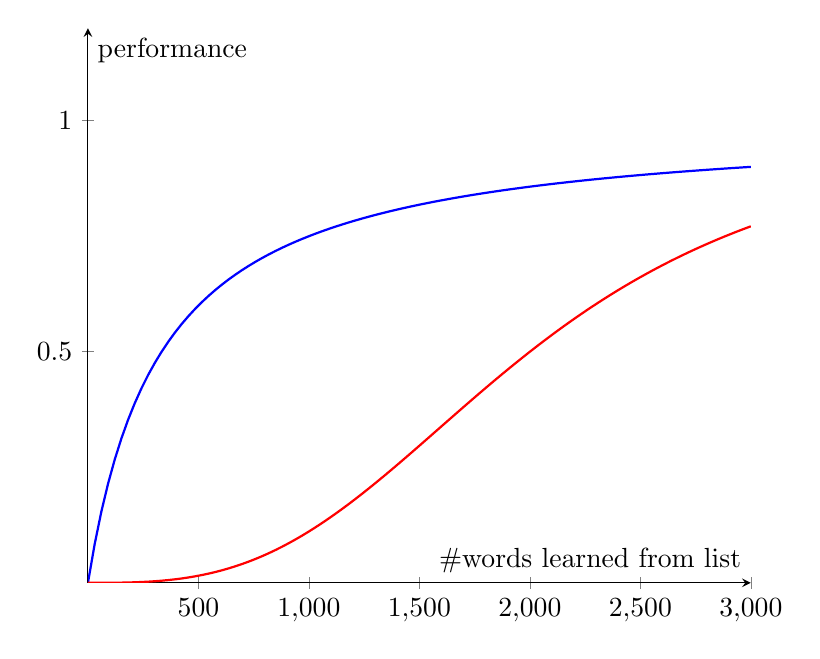
\begin{tikzpicture}
		\begin{axis}[
				axis lines = middle,
				xlabel = {\#words learned from list},
				ylabel = {performance},
				xtick = {0,500,1000,1500,2000,2500,3000},
				ytick = {-1,-0.5,0,0.5,1},
				samples = 100,
				domain = 0:3000,
				ymax=1.2,
				width=10cm
			]

			%curve
			\addplot[blue, thick] {1 - (1/((0.003*x)+1)};
			\addplot[red, thick] {1 - (1/(((0.0005*x)^3)+1)};
		\end{axis}
	\end{tikzpicture}
	\caption{Visualization of vocabulary list efficiency: \textbf{\textcolor{blue}{Blue}} represents the score with learning with an efficient list, \textbf{\textcolor{red}{Red}} represents the score learning from a less efficient list (i.e, less useful words at the top of the list)}
	\label{fig:voc-list-efficiency}
\end{figure}

\section{Experimental Setup: Measuring Word Utility as Ability Improvement in Humans} \label{sec:human-efficiency-testing}

\contentdescription{State utility in terms of language ability improvement
	aim is not just to evaluate, but also efficiently find lists of vocab
	give problems that is faced when trying to test this approach with human test subjects: no repeatability, high costs
}

With the formula \ref{eq:optimal-vocab-list}, we now have set our goal more concretely.
We are left with the question of how to design an actual experiment to test vocabulary list efficiency, and also how to generate one that is approximates an optimal list.
Hence, this section lays forth a hypothetical experiment design by using a human test subject to test efficiency, which will, however, be found to suffer from problems of feasibility, which the following section will set out to solve.

\subsubsection{Experimental Setup}
Let us first consider an example scenario, where we wish to measure the efficiency of one vocabulary list $l_A$ at $k=200$, $k=500$ and $k=2000$ words:
First, we would need to find a human test subject $s$ who does not know any words of the target language at the outset.
We then make the subject learn the words from $l_A$ one by one.
Once the subject seems to know 200 words, we perform a language exam and note their score.
Finally, we repeat the process for 500 and 2000 words.

\subsubsection{Problems of the Setup}
While this test setup might take a long time to complete for high $k$ values, it is still feasible.
But if we wish to compare the efficiency of $l_A$ with a second list $l_B$, we must measure how the same subject performs if they learn from the second vocabulary list, which presents is an unavoidable issue:
\textbf{The test subject cannot arbitrarily forget the words they have learned from the first list $l_A$.}
The experiment is thus not repeatable.

If we tweak the experiment such that each vocabulary list is learned by a different test subject, we introduce differences in capabilities between test subjects, making the evaluation of the list's efficiencies much more complicated to measure.
To make up for these inconsistencies, we might boost the number of test subjects to the point where each list is learned by a statistically significant group of subjects, but this would cause a sharp increase in the cost of the experiment.

However, this theoretical test setup could be feasible using a non-human test subject:
Using AI models and Explainable AI to analyze their interaction with language, we could not only evaluate, but even compile lists with drastically reduced costs.
This approach is laid out in the following sections.

\section{Experimental Setup with AI Model} \label{sec:experimental-setup-with-ai}
\contentdescription{I view AI models as containers of language knowledge. We can perform studies on it as though it were human, gaining knowledge "from the viewpoint of an entity interacting with language"}

This work is interested in finding vocabulary lists that language learners can use to gain linguistic competence in their chosen field in the least possible time.
Section \ref{sec:formal-problem-statement} has specified how with the help of a proxy task, we can define this efficiency.
Section \ref{sec:human-efficiency-testing} has suggested a hypothetical experiment for testing the efficiency of a vocabulary list with human test subject.
However, we have established that the experiment is not easy to set up consistently, as it cannot be repeated with the same test subject on different lists, and a large pool of test subjects either means lower comparability of the scores or significantly increased costs.

To circumvent this issue, this work proposes the following idea:
To replace the human test subject in the experiment described in Section \ref{sec:human-efficiency-testing} with an AI model, facilitating a consistent and economical setup.

The following paragraphs will lay out how, in such a setup, we can model the concepts from Section \ref{sec:statement-of-goal} such as linguistic context and utility with technological tools.

\subsubsection{AI as a Test Subject} \label{sec:ai-as-test-subject}
In recent years, AI models such as ChatGPT \tocite{cite ChatGPT} or BERT \tocite{cite BERT} have become highly adept at fulfilling language-related tasks such as Language Modeling \tocite{LLMs}, Named Entity Recognition and Sentiment Detection.

Such models possess as level of "understanding" that extends to the meaning of words:
They can recognize that two words such as "building" and "apartment" are close to each other in meaning, even though the words are dissimilar on a character level (this work makes no claims as to whether this understanding is real to that of a human, only that the models behaves as though it were).
Thanks to this semantic language "understanding", AI models surpass the purely statistical approaches that were the paradigm of NLP until recently \tocite{paper contrasting traditional with AI approaches}.
Thus, instead of a human performing a language exam to increases in linguistic understanding (\textit{utility}), we could let an AI model perform an NLP task on a corpus instead.

If we run the model on a specific corpus and mask some of the words in the input, it is expected that the performance will decrease in comparison to the full input.
However, presumably some words will have a larger impact on the performance than others.
If we view removing words from the input as the equivalent of a human not knowing a word in a text, this performance differential can be a proxy metric for word utility and for human language ability.

\subsubsection{Modified Experimental Setup with AI}
With this new proxy metric for word utility in mind, we can propose a new experiment.
To test the efficiency of a vocabulary list, we modify the setup from \ref{sec:human-efficiency-testing} as follows:

Let a pre-trained AI model perform its NLP task on a corpus.
At the start, we mask all the tokens in the input to simulate a language learner who is a complete beginner and thus knows no words in their target language.
We then progressively unmask the words from the vocabulary list in the input, and each time run the AI on the corpus to check the updated (and presumably improved) performance.

This will yield a plot of performance over unmasked words which will tell us how quickly the performance improves with unmasked words, similar to Figure \ref{fig:voc-list-efficiency}.
A quickly increasing performance will correspond to an efficient vocabulary list, whereas an inefficient list will create a plot with low initial gains in performance.

The modified experiment addresses the two issues proposed with the original setup:
It is cheap when compared to using a human test subject and unlike the human, the AI model has no memory of previous tests, meaning we can run the experiment consistently every time.


Next, let us see how the components in this setup interact with each other to model the concepts introduces in Section \ref{sec:statement-of-goal}:

\subsubsection{Influence of Components on Result}
The evaluation of the vocabulary list efficiency in the experiment will depend on the following components:

\begin{itemize}
	\item The AI model employed
	\item The input corpus
	\item The NLP task used
\end{itemize}

We have already addressed the role of the AI model in Section \ref{sec:ai-as-test-subject}.
The corpus and the NLP task performed by the model will also influence how quickly the AI model's performance increases with a given vocabulary list:

For example, when performing Sentiment Detection, words relating to emotion such as "hate", "like", "amazing" will matter more than if for an Information Retrieval task such as Temporal Tagging.

The corpus will have a more obvious influence on the performance, since corpora differ in many aspects such as formality, topic, and format of the text, all of which are components of a linguistic context.

Thus, by using diverse corpora, we can model various language contexts, and test word utility in those contexts.
Once we have efficient vocabulary lists across those contexts, a language learners could choose one or several of these lists, based on what linguistic context is closest to their language learning goals.


Table \ref{table:concept-implementation-correspondence} summarizes the correspondences between the concept and the technical component.

\begin{table}[ht]
	\centering
	\begin{tabularx}{\textwidth}{|X|X|}
		\hline
		\textbf{Abstract concept} & \textbf{Technical Implementation}  \\
		\hline
		Test subject              & AI model                           \\
		\hline
		Language ability          & Performance in NLP task            \\
		\hline
		Language context          & Corpus                             \\
		\hline
		Word utility              & Impact of word on task performance \\
		\hline
	\end{tabularx}
	\caption{Correspondence of abstract concepts to parts of implementation.}
	\label{table:concept-implementation-correspondence}
\end{table}

The next section will tackle the problem of how to not only test list efficiency, but make lists that approach an optimally efficient list.

\section{Evaluating vs. Making Lists of Useful Vocabulary} \label{sec:eval-vs-creation}
The previous section describes an approach for evaluating the efficiency of vocabulary lists, which measures how quickly the list lets a learner improve their understanding in a specific context.
While it can be seen as an improvement on the human setup because of its improved consistency and economy, it describes only the process of evaluation, not generation.
Actually finding optimal vocabulary lists is theoretically possible by testing every possible vocabulary list with all words in the language.

In practice, however, this would require an enormous amount of computational resources, as can be seen on a simple example:

Let us suppose we wish to find the most efficient vocabulary list of 1,000 words for some context.
To speed up list generation, we can make a preselection by allowing only the most frequent 20,000 words in the context as candidate members of this list.
This would yield a total number of $P(20000, 1000) = \frac{20000!}{19000!}$ possible vocabulary lists, all of which would need to be tested for efficiency to find the most efficient one.

We can optimize the evaluation process, however, since these tests consist of running the proxy task with a gradually increasing vocabulary, and each vocabulary will be used in the evaluation for many vocabulary lists.
For our example, a vocabulary is a set of words formed by taking the first $n$ elements of the vocabulary list where $n \in [0, 1000]$.
If we only consider the number of possible vocabularies with a cardinality between 0 and 1,000, we get
$
	\sum_{k=0}^{1000} \binom{20000}{k} \approx \frac{1}{2} \times 2^{20000} = 2^{19999}
$ runs of the proxy task. Clearly, this is still an unfeasible amount of computation.

It can thus be seen that finding optimal vocabulary list is much too expensive when performed with a brute-force approach.
For this reason, the next section will introduce an alternative method for finding efficient lists of vocabulary, based on XAI as a tool which extracts information about the linguistic skills of AI models.

\section{Generating Efficient Lists of Vocabulary} \label{sec:list-generation}

The previous sections have shown the challenges in evaluating the efficiency of vocabulary lists with human test subjects, and suggested a repeatable approach utilizing AI models, NLP tasks and corpora to overcome these challenges.
We have seen, however, that this approach does not suffice to generate efficient vocabulary.
Therefore, to achieve cost-efficient list generation, this section advocates for adding a final component to our experimental setup, namely Explainable AI.

\subsubsection{Explainable AI as a Tool of Analysis} \label{sec:xai-as-tools-of-analysis}
The guiding question of this thesis is:
\textit{Which words provide the most language understanding in a given linguistic context?}.
Section \ref{sec:experimental-setup-with-ai} has put forward an experimental setup in which the concepts of language understanding and context are simulated with technological components.
By substituting these terms, the question is turned into:
\textit{Which words provide the highest improvements in performance of an AI model performing an NLP task on a given corpus?}.

Put like this, the question is very close to the questions that the field of Explainable AI seeks to answer.
A typical question of Explainable AI would be:
\textit{Why, for a given input, does the model arrive at its output?}. \tocite{Definition of XAI. How to not make this seem like a direct quote?}
To be more precise, this is a question for a \textit{local} explanation (see Section \ref{sec:xai-methods}).
As mentioned in Section \ref{sec:xai-methods}, we will use Feature Attribution methods, which for an NLP task transform the question into:
\textit{Which words in the input have the most influence on the model arriving at its output?}

By answering this question on a statistically relevant sample of individual inputs from a corpus, we can find out which words are the most essential for the AI model to perform its task in the corpus overall.
If the words found in this way are close to those that would provide the most utility to a human learner as well, they could be used to create very efficient vocabulary lists as well.

Once we have calculated the utilities of words, we only need to sort the words by their utility to arrive at a vocabulary list that should be close to optimally efficient.
It must be noted that this is only an approximation of a maximally efficient list.
This is because, theoretically, the utility of two words combined could be higher than the sum of their individual utilities.
In other words, our approach ignores possible synergistic effects between words.

By adding XAI as a tool for analyzing the interaction of the AI model with the corpus, we finally have an experimental setup for generating efficient vocabulary lists.
This is not a replacement of the approach described in Section \ref{sec:ai-as-test-subject}.
Rather, this work will use the generation approach to make lists (Chapter \ref{ch:implementation}), and the evaluation approach for testing which method leads to the most efficient lists (Chapter \ref{ch:evaluation}).

In the next section, we will tackle the implementation of this approach.
We will present various choices for these components, and argue for some to be used over others, with the aim of making the utility estimated by the framework align as much as possible with utility to human learners.

%
% It is readily seen that these components are not independent of each other.
% Some completely determine the choice of another, while others limit the selection of the other components.
% 	[describe dependencies between components]
% Task $\rightarrow$ model $\rightarrow$ tokenizer $\rightarrow$ words.
%
% must investigate comparability of results later.

% (also corpus $\rightarrow$ task)
% \subsection{Preliminary Investigations of Integrity}
% The core idea this work is to evaluate word utility by investigating a function (in the form of an AI model) that presumably represents some level of understanding of the language and checking which inputs (words) have the biggest influence on either the input or the model's internal state.
% To ensure the function does possess this understanding, it is necessary to first ensure that the output of the model corresponds reliably to the ground truth, in other words, to tests the performance of the model on the specific data that will later be used to investigate the model itself.
%
% \todo{A lot of prelim. test results, for example, first tests of NSP model on opensubs sentences show low reliability. Might also have to move this section to end (or in "results" chapter?)}
%


%
%
% \section{Experimental Setup with AI Technology}
% With the experimental setup described in chapter \ref{seq:human-efficiency-testing}, we established a way to test the efficiency of a vocabulary list with a human test subject.
% Now that we have introduced the idea of performing the experiment with an AI model instead, let us examine how such an approach would work:
% Chapter \ref{table:concept-implementation-correspondence} suggested ways that we could use technological components to stand in for abstract concepts.
%
%
% \todo{ restate math problem definition with components replaced by AI}
%
%

% \section{TO BE MOVED OR DELETED}
% Let us examine examples of how utility may be defined:
% In the question "Would you like some coffee?", the most important part is "coffee".
% If we replaced the entire sentence with "coffee?", the meaning becomes less clear, but it is still possible to guess what is meant.
% If, however, we replace the sentence with "would?", there is so little information in the sentence that it becomes impossible to guess the meaning.
% To identify which words are important to understand the question, we could ask a human to point them out.
% However, this is not very quantifiable and the answer is likely to be influenced by bias.
% We could try removing some of the words in the sentence and see if a human hearing the question can still answer appropriately.
% While this removes some of the bias, there are still issues with this approach:
% Going through all possible permutations of the sentence would take a great amount of time to perform, and the same test subject cannot process one permutation without being influenced by the past experiences:
% If we go through "would?", "you?", "like?", "some?", "coffee?" in sequence, the test subject would have full knowledge of the sentence by the time the last item is asked.
% These problems can be alleviated by using AI models: They are cheaper to perform tests on than humans, and can be employed in such a way as to answer the question without being influenced by the previous questions each time.
%
% \todo{Explain approach where a model is trained on small set of words and performance is evaluated. But too costly.}
%
%
% While the models achieving state-of-the-art performance (neural networks) are black boxes for the most part, they are easier to understand than human decisions and the field of Explainable AI has produced various approaches to gauge the importance of inputs to the model.
% Explainable AI has the explanation of the decisions of AI models as its aim.
% This means that when analyzing the decisions of AI models by reducing them to human-understandable rules or by observing which words are the most important for the AI to fulfill its tasks, we are not technically observing rules of objective truth, but only the behavior which the AI has learned to perform its task.
% If we try to extract truthful knowledge about language from the AI, we are relying on the assumption that the AI has learned rules that correspond to linguistic reality.
% However, in the case of state-of-the-art models, we know the performance of such models to meet certain standards, which supports the above assumption.
%
